
%%%%%%%%%%%%%%%%%%%%%%% file typeinst.tex %%%%%%%%%%%%%%%%%%%%%%%%%
%
% This is the LaTeX source for the instructions to authors using
% the LaTeX document class 'llncs.cls' for contributions to
% the Lecture Notes in Computer Sciences series.
% http://www.springer.com/lncs       Springer Heidelberg 2006/05/04
%
% It may be used as a template for your own input - copy it
% to a new file with a new name and use it as the basis
% for your article.
%
% NB: the document class 'llncs' has its own and detailed documentation, see
% ftp://ftp.springer.de/data/pubftp/pub/tex/latex/llncs/latex2e/llncsdoc.pdf
%
%%%%%%%%%%%%%%%%%%%%%%%%%%%%%%%%%%%%%%%%%%%%%%%%%%%%%%%%%%%%%%%%%%%


\documentclass[runningheads]{llncs}

\usepackage{amssymb}
\usepackage{amsmath}
\usepackage{amsfonts}
\setcounter{tocdepth}{3}
\usepackage{graphicx}
\usepackage{wrapfig}
\usepackage{multirow}
\usepackage{url}

%\urldef{\mailsa}\path|{alfred.hofmann,ursula.barth,ingrid.beyer,natalie.brecht,|
%\urldef{\mailsb}\path|christine.guenther,frank.holzwarth,piamaria.karbach,|
%\urldef{\mailsc}\path|anna.kramer,erika.siebert-cole,lncs}@springer.com|
\newcommand{\keywords}[1]{\par\addvspace\baselineskip
\noindent\keywordname\enspace\ignorespaces#1}
%\renewcommand{\familydefault}{\sfdefault}
%\documentclass{llncs}
%
%\pagestyle{headings}
%\usepackage{amsmath}
\newcommand{\new}{\newcommand}
\new{\bg}{\begin}
\new{\lp}{\left(}
\new{\rp}{\right)}


\newcommand{\xx}{\mathcal{X}}
\newcommand{\yy}{\mathcal{Y}}
\newcommand{\rr}{\mathbb{R}}

\new{\iii}{\begin{enumerate}}
\new{\fff}{\end{enumerate}}
\new{\iiii}{\begin{itemize}}
\new{\ffff}{\end{itemize}}
\new{\mfi}{\begin{eqnarray*}}
\new{\mff}{\end{eqnarray*}}
\new{\mfni}{\begin{eqnarray}}
\new{\mfnf}{\end{eqnarray}}
\new{\beeq}[2]{\begin{equation}\label{#1}{#2}\end{equation}}
\new{\eqn}[1]{~(\ref{#1})}

\new{\room}{\ \ \ \ }
\new{\card}{\#}


\new{\nor}[1]{\|{#1}\|}
\new{\normi}[1]{\left\|{#1}\right\|_{\infty}}
\new{\scal}[2]{\left\langle{#1},{#2}\right\rangle}
\new{\scalh}[2]{\left\langle{#1},{#2}\right\rangle_\hh}
\new{\set}[1]{\{{#1}\}}
% GENERAL MACRO
%%%%%%%%%%%%%%%%%%%%%%%%%%%%
%\new{\rone}{{\mathrm{I\hskip-2.2pt R}}}
\new{\com}{{\mathbb C}}
\new{\rone}{{\mathbb R}} 
\new{\nat}{{\mathbb N}}

\new{\fz}{f_\vz}
\new{\fzlo}{\overline{f}_\vz^\la}
\new{\rd}{\rone^\dm}
\new{\ed}{{\mathbb E}}
%\new{\nat}{{\mathrm{I\hskip-2.2pt N}}}
%\new{\com}{{\mathrm{I\hskip-2.2pt C}}}

%
%\new{\rd}{{\mathrm{I\hskip-2.2pt R}}^\dm}
%\new{\ed}{{\mathrm{I\hskip-2.2pt E}}^\dm}
\new{\argmin}{\operatornamewithlimits{argmin}}
\new{\argmax}{\operatornamewithlimits{argmax}}
\new{\Prob}[1]{\mathrm{P}\left[\, #1 \right]}
\new{\E}{{\mathbb E}}
\new{\eps}{\varepsilon}
%\new{\nor}[1]{\left\|{#1}\right\|}
%\new{\scal}[2]{\left\langle{#1},{#2}\right\rangle}

%LEARNING MACRO
%%%%%%%%%%%%%%%%%%%%%%%%%%%%%
\new{\marg}{\rho_X}
\new{\prob}{\rho}
\new{\dm}{d}
\new{\tr}{\vz}
\new{\n}{n}
\new{\vb}{{\mathbf b}}
\new{\vf}{{\mathbf f}}
\new{\vl}{\bar{\ell}}
\new{\vx}{{\mathbf x}}
\new{\vy}{{\mathbf y}}
\new{\vz}{{\mathbf z}}
\new{\vc}{{\mathbf c}}
\new{\vu}{{\mathbf u}}
\new{\vv}{{\mathbf v}}
%\new{\k}{{\mathcal k}}
%\new{\kx}{{\mathcal k}_x}
\new{\kk}{K}
\new{\s}{K^s}
\new{\kkx}{K_x}
\new{\w}{W}
\new{\wx}{\w_x}
\new{\WW}{{\mathbf W}}
\new{\DD}{{\mathbf D}}
\new{\LL}{{\mathbf L}}
\new{\LS}{{\mathbf L}_{s}}
\new{\LR}{{\mathbf L}_{r}}
\new{\II}{{\mathbf I}}
\new{\KK}{{\mathbf K}}
\new{\ka}{\kappa}
\new{\ls}{\ell}
\new{\err}{{\mathcal E}}
\new{\emp}{{\mathcal E}_z}
\new{\hh}{{\mathcal H}}
\new{\oo}{{\mathcal G}}
\new{\ff}{{\mathcal F}}
\new{\ldue}{L^2(X,\rho)}
\new{\la}{\lambda}
\new{\dd}{\delta}
\new{\vG}{{\mathbf \Gamma}}
\new{\vC}{{\mathbf C}}
\new{\vS}{{\mathbf S}}
\new{\vU}{{\mathbf U}}
\new{\vY}{{\mathbf Y}}
\new{\vX}{{\mathbf X}}
\new{\vaa}{{\boldsymbol{\alpha}}}
\new{\bh}{{\mathcal B}(\hh)}
\new{\hs}{ HS(\hh)}

\new{\lduew}{L^2(X,\rho_\w)}
\new{\Tt}{L_{K,\hh}}
\new{\Tn}{L_{K,n}}
\new{\U}{U_\w}
\new{\LK}{L_{K}}

\new{\Wt}{L_{\w,\hh}}
\new{\Wn}{L_{\w,n}}

\new{\Ah}{A_{\hh}}
\new{\An}{A_{n}}

\new{\Ls}{L_{s}}
\new{\Lr}{L_{r}}

\new{\Lshn}{L_{s,\hh,n}}
\new{\Lrhn}{L_{r,\hh,n}}
\new{\LLsh}{L_{s,\hh}}
\new{\LLrh}{L_{r,\hh}}
\new{\I}{I_{\kk,\w}}
\new{\Ik}{I_\kk}
\new{\IIk}{I^*_\kk}
\new{\Iw}{I_\w}
\new{\IIw}{I^*_\w}

\new{\m}{m}
\new{\mn}{m_{n}}

\new{\Ax}{{A_{\mathbf x}}}
\new{\A}{A}
\new{\AR}{\A^\la}
\new{\ARx}{\A^\la}
%\new{\Tx}{{T_{\mathbf x}}}
\new{\Tx}{L_{K,n}}
%\new{\Sx}{{S_{\mathbf x}}}
\new{\Sx}{{S_n}}
\new{\T}{T}
\new{\Kx}{{K_{\mathbf x}}}
\new{\K}{K}
\new{\g}{{\mathcal G}}
\new{\sn}{\hat{\sigma}}
\new{\vn}{\hat{v}}
\new{\un}{\hat{u}}

\new{\so}{{s^\prime}}

\new{\Pj}{P_j}
\new{\Qj}{Q_j}
\new{\Pnj}{\hat{P}_j}
\new{\Qnj}{\hat{Q}_j}

\new{\cl}{c}
\new{\br}{b}
\new{\R}{R}
\new{\vre}{\vf_\rho}
\new{\re}{f_\rho}
\new{\X}{\mathcal X}
\new{\Y}{\mathcal Y}
\new{\W}{\mathcal W}

\new{\bbeta}{\boldsymbol{\beta}}
%END  command MACRO----------------------------------



\begin{document}

\mainmatter  % start of an individual contribution

% first the title is needed
\title{Towards a theoretical framework for learning multi-modal patterns for embodied agents}

% a short form should be given in case it is too long for the running head
% \titlerunning{Lecture Notes in Computer Science: Authors' Instructions}

% the name(s) of the author(s) follow(s) next
%
% NB: Chinese authors should write their first names(s) in front of
% their surnames. This ensures that the names appear correctly in
% the running heads and the author index.
%
% \author{...%
% \and ...\and ...\and ...}
\author{AUTHORS}
%
% \authorrunning{Lecture Notes in Computer Science: Authors' Instructions}
% (feature abused for this document to repeat the title also on left hand pages)

% the affiliations are given next; don't give your e-mail address
% unless you accept that it will be published
% \institute{institute...,\\
% ...\\
% mail...\\
% \mailsa\\
% \mailsb\\
% \mailsc\\
% \url{...}}

\institute{AFFILIATIONS}
%
% NB: a more complex sample for affiliations and the mapping to the
% corresponding authors can be found in the file "llncs.dem"
% (search for the string "\mainmatter" where a contribution starts).
% "llncs.dem" accompanies the document class "llncs.cls".
%

% \toctitle{Lecture Notes in Computer Science}
% \tocauthor{Authors' Instructions}
\maketitle


\begin{abstract}
% The abstract should summarize the contents of the paper and should
% contain at least 70 and at most 150 words. It should be written using the
% \emph{abstract} environment.

Multi-modality is a fundamental feature that characterizes biological systems 
and lets them achieve high robustness in understanding skills while coping with
uncertainty.
Relatively recent studies showed that multi-modal learning
is a potentially effective add-on to artificial systems, allowing
the transfer of information from one modality to another.
In this paper we propose a general architecture for jointly learning visual and motion patterns: 
by means of regression theory we model a mapping between the two sensorial modalities improving 
the performance of artificial perceptive systems.
We present promising results on a case study of grasp classification in a controlled setting
and discuss future developments. 

\keywords{ multi-modality, visual and sensor-motor patterns, regression theory, behavioural model, objects and actions recognition 
% We would like to encourage you to list your keywords within
% the abstract section
}
\end{abstract}

 Introduced in the early 90s by Boser, Guyon and Vapnik \cite{BGV92},
\emph{Support Vector Machines} (SVMs) are a class of machine learning
algorithms deeply rooted in Statistical Learning Theory
\cite{v-edbed-82}, able to classify data taken from an unknown
probability distribution, given a set of training examples. As opposed
to analogous methods such as, e.g., artificial neural networks, they
have the main advantages that $(a)$ training is guaranteed to end up
in a global minimum, $(b)$ their generalization power is theoretically
well founded, $(c)$ they can easily work with highly dimensional,
non-linear data, and $(d)$ the solution achieved is sparse. Due to
these good properties, they have been now extensively used in, e.g.,
speech recognition, object classification and function approximation
\cite{Cristianini00}. On the other hand, one of their main drawbacks
is their alleged inability to cope with large datasets
\cite{KeerthiCDC06}.

Yet, in most real-life applications, datasets \emph{are} large, for
example when online learning must be performed. Online learning is a
scenario in which training data is provided one example at a time, as
opposed to the batch mode in which all examples are available at once
(see \cite{Laskov2006} and citations therein). In the case of, e.g.,
non-stationary data, online algorithms will generally perform better
since ambiguous information (i.e., whose distribution varies over
time) is present, and couldn't possibly be taken into account by the
batch algorithm. Online algorithms allow to incorporate additional
training data, when it is available, without re-training from scratch.

In an online setting there is no guarantee that the flow of data will
\emph{ever} cease; therefore, applying SVMs here looks appealing but
we need a way to cope with large datasets. One of the keys to the
problem seems to lie in  the sparseness of their solution. That an
SVM solution is \emph{sparse} means that usually just a few samples
account for its complexity; in fact, SVMs can be seen as a way of
compressing data by selecting ``the most important'' samples
(\emph{support vectors}, SV) among those in the training set. Keeping
the number of SVs small without losing accuracy is therefore a major
challenge, also since a recent result \cite{Steinwart03} shows that
their number grows indefinitely with (namely, proportionally to) the
number of training samples.

In this paper we propose a method of incrementally selecting SVs based
upon \emph{linear independence in the feature space}: SVs which are
linearly dependent on already stored ones are rejected, and a smart,
incremental minimization algorithm is employed to find the new minimum
of the cost function. The size of the kernel matrix (the core of an
SVM and its major bottleneck) is therefore kept small. Our experiments
indicate that SVMs employing this idea, that we call
\emph{Online Independent Support Vector Machines} (OISVMs), do not
grow linearly with the training set, as it was the case in
\cite{Steinwart03}, but reach a limit size and then stop growing
\cite{engel2004}. In the case of finite-dimensional feature spaces
they also \emph{keep the full accuracy of standard SVMs}; whereas in
the infinite-dimensional case, at the price of a negligible loss in
accuracy, one can tune the growing rate of the machine.

To support this claim, we show an extensive set of experimental
results obtained by comparing SVMs and OISVMs on standard benchmark
databases as well as on a real-world, online application coming from
robotic vision: place recognition in an indoor environment, from
sequences acquired by robot platforms under different weather
conditions and across a time span of several months. Our results show
that, on standard benchmarks, the accuracy of OISVMs can be up to only
$0.063\%$ worse than SVMs, with less than $5\%$ of the support
vectors; whereas, on the real-world application, we get as few as one
third of the SVs required by an online approximated method, while
retaining essentially the same accuracy.

The paper is structured as follows: after a review of the relevant
literature, Section \ref{sec:bg} gives an overview of background
mathematics proper to SVMs; in Section \ref{sec:opt} OISVMs are
described.  Section \ref{sec:exp}  shows the experimental results
and lastly, in Section \ref{sec:concl}, conclusions are drawn and future
work is outlined.



\begin{figure}[h!]
	\centering
	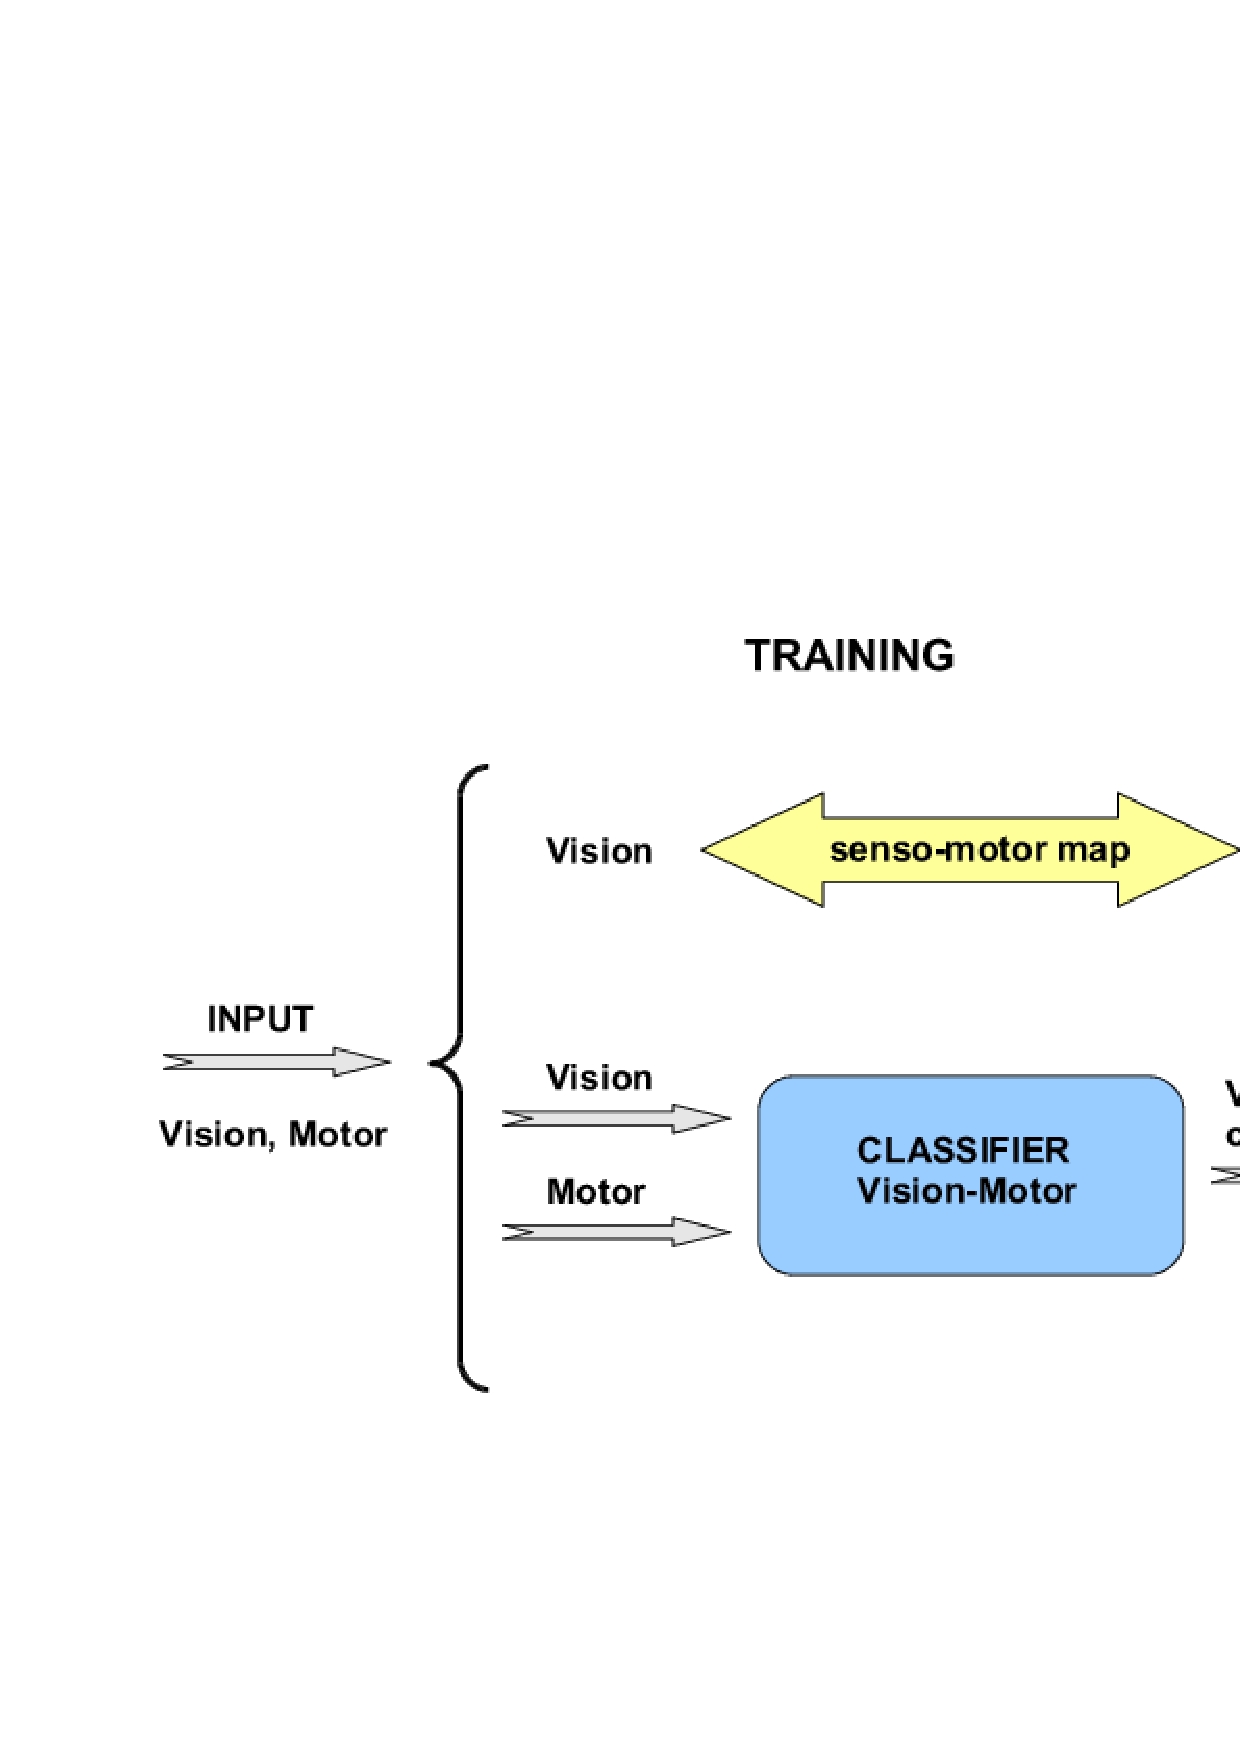
\includegraphics[width=0.7\textwidth]{images/train_fig}
	\caption{blabla}
	\label{fig:training-scheme}
\end{figure}

\begin{figure}[h!]
        \centering
        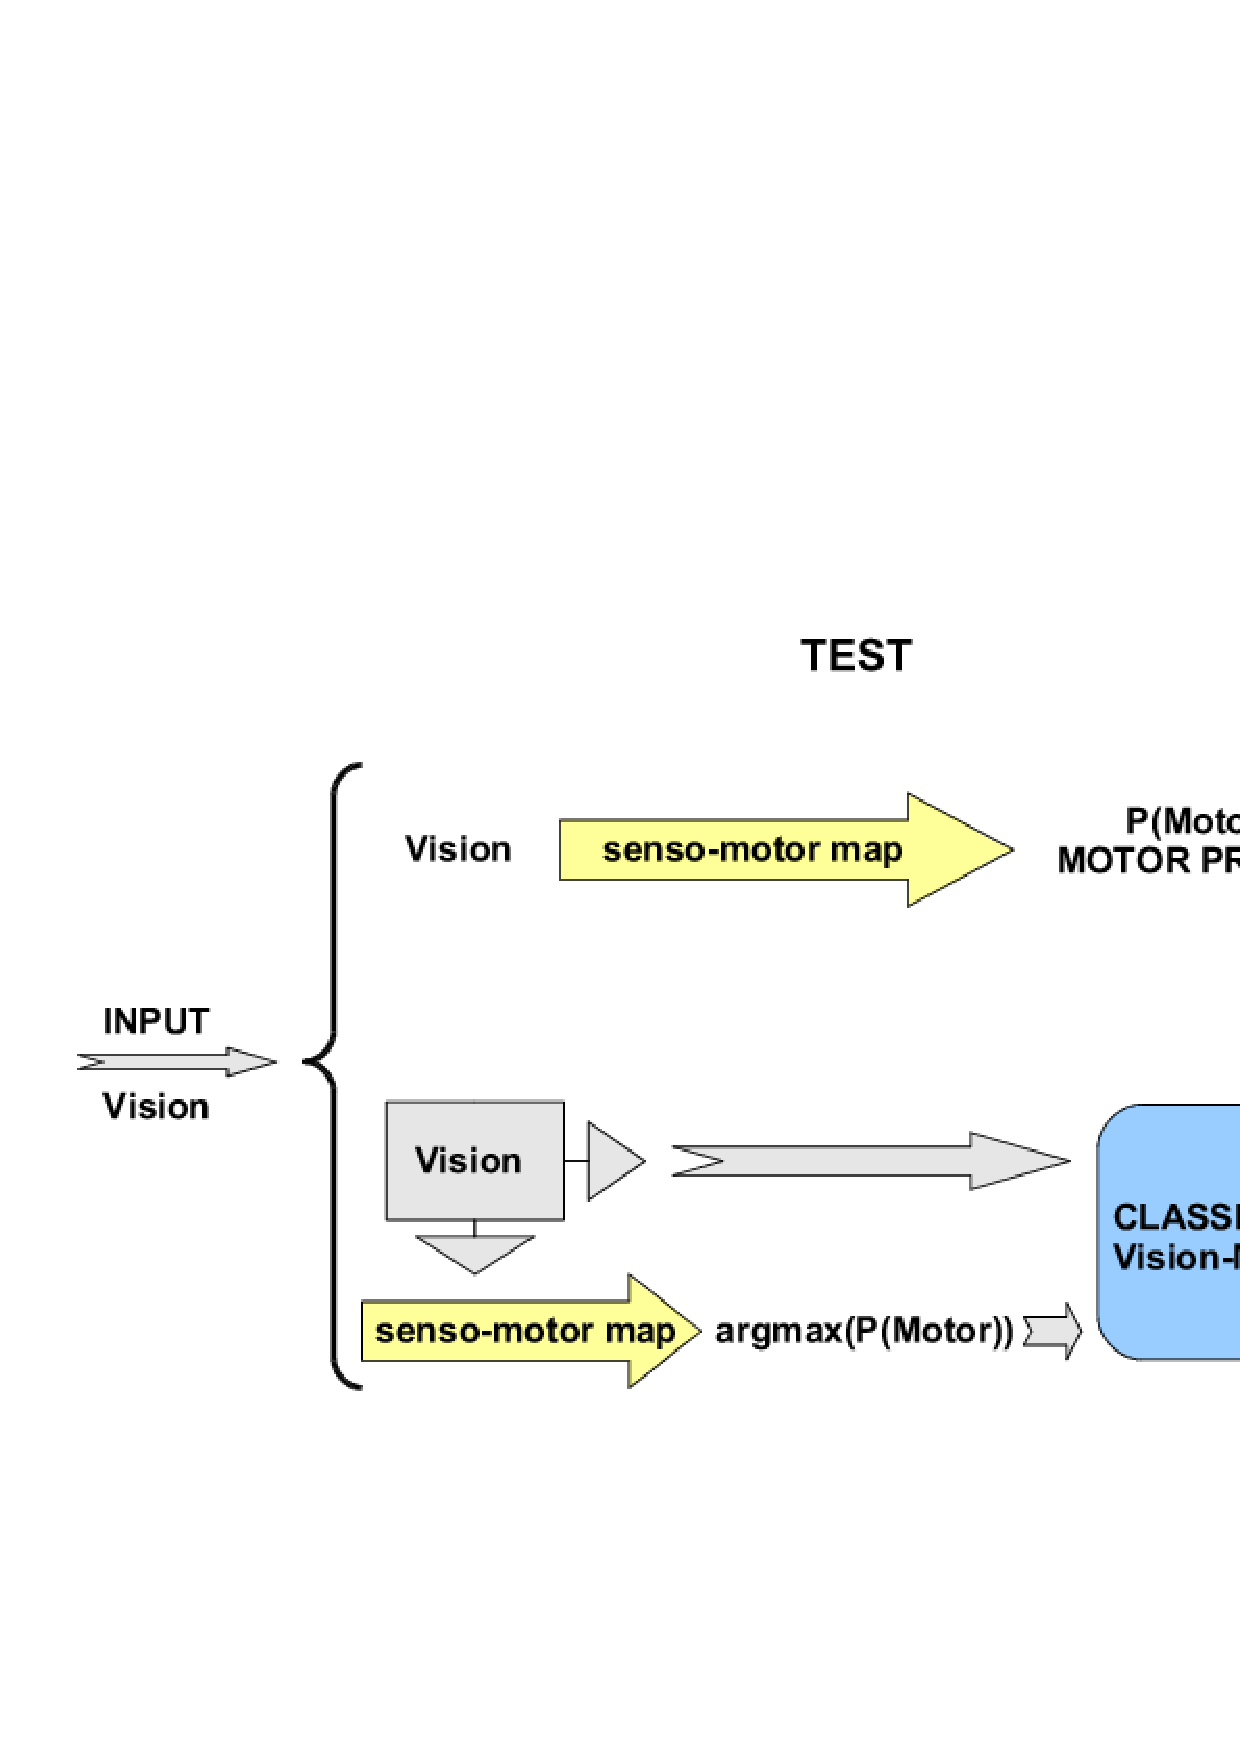
\includegraphics[width=0.7\textwidth]{images/test_fig}
        \caption{blabla}
        \label{fig:test-scheme}
\end{figure}


%\vskip -0.5cm

The training phase is schematically illustrated in Figure \ref{fig:training-scheme}. During training, the system receives as input labeled visual and motor
perceptual representation. These correspond to the seen object (Visual Perceptual Representation, VPR) and to the grasp posture of the hand
manipulating the object (Motor Perceptual Representation, MPR). On these data, the system builds in parallel two functions: a senso-motor map
between VPR and MPR (Figure \ref{fig:test-scheme}, top) and a classification function receiving as input both modalities, trained
to recognize the perceived object (Figure \ref{fig:training-scheme}, bottom). Technical details on how we compute the sensor motor map and the
multi-modal classifier are reported in section .. and ...

Figure \ref{fig:test-scheme} shows the test phase with its two possible outcomes. When receiving as input a VPR of a known object, the system can
opt for two different types of action:
\begin{itemize}
\item {\em Activation of the sensor-motor map}. This produces as an output an estimate of the most probable motor grasps associated 
to that object, with the corresponding 
MPRs for the grasp postures. We call this estimates {\em motor priming}, as they would correspond in an embodied agent to the pre-activation of the possible 
grasps. A detailed description of how we obtain the motor priming is given in section .....

\item {Object classification}. Note that, having learned the object on two modalities, the classifier needs as input a VPR and its corresponding MPR. We derive the
{\em not perceived} MPR using the senso-motor map (Figure \ref{fig:test-scheme}, bottom). The obtained motor priming is then given as input to the classifier with the VPR. We stress again that the clasifier recognizes the object on the basis of its visual appearance and of how it can be grasped. Experiments
reported in section ... shows clearly that this leads to a significant increase in performance compared to using only visual information.

\end{itemize}

{\bf FIXM EBABS; NICOLETTA; CLAUDIO: io metterei qui la descrizione delle visual and sensomotor features, senza farci una sezione specifica per ognuna}


\begin{figure}
	\centering
	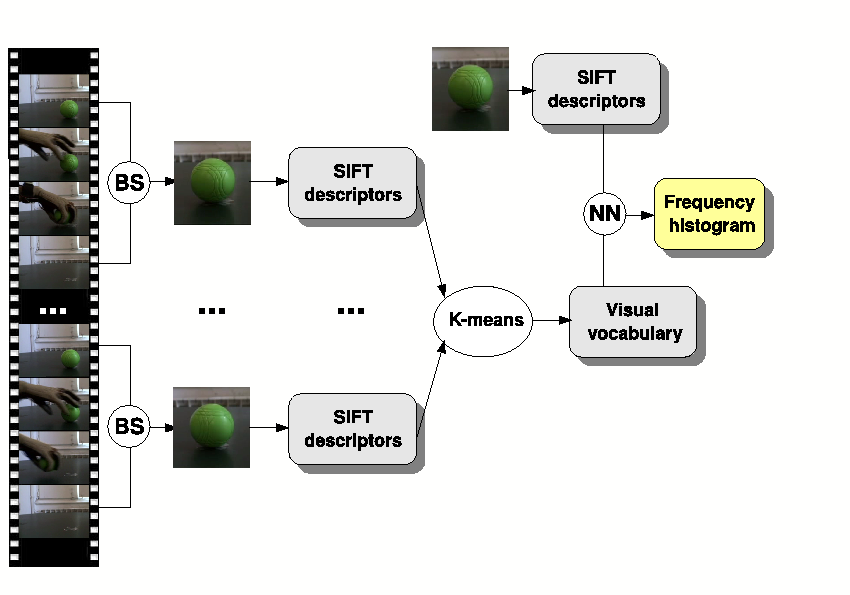
\includegraphics[width=0.8\textwidth]{images/schema_vision}
	\caption{A schema of the vision unit. First, suitable frames are extracted from the sequence and objects are located by means of background subtaction (BS). SIFT descriptors of a set of random points are input of a clustering step to get to the final visual vocabulary. Finally, each image is represented with respect to the vocabulary adopting a nearest neighbour (NN) strategy (see text for details).}
	\label{fig::vision}
\end{figure}

\section{Vision unit}
\label{sec::vision}
As we will discuss in Sec. \ref{sec::experiments}, the system gathers, as one input, a video sequence acting as {\it spectator}, whose focus is on object appearance. The goal of the vision unit is to process the signal to obtain a global model of a set of given objects.
Figure \ref{fig::vision} shows the pipeline of the vision unit when considering only one object (the same procedure is applied to the whole set of objects). Among the sequence, we first select the frames showing only the object  without any occlusion, then we locate more precisely its position by means of a simple background subtraction. 
Although in our application there is not an explicit object recognition step, it is clear from the architecture pipeline that a robust and specific object model is functional to subsequent analysis. It is worthwhile also to mention that with the terms {\it object recognition} we indicate the characterization of a specific object instance (againts the concept of categorizing classes of objects).
We adopt an approach based on local features to describe image structures: because of their popularity a rich variety of local measurements have been proposed in the literature \cite{harris,schmid,lowe} and applied successfully to objects recognition and categorization problems (see \cite{csurka,ferrari} just to name a few). 
Local approaches tipically include two distinct steps: keypoints extraction and description. 
However, in our case, a keypoint based-representation often ends up into a poor description
due to the limited size of the images. We thus built our representation by extracting enough 
random points  guaranteeing a more homogenous sampling.
We chose to adopt SIFT descriptors \cite{lowe,schmid2} to model image patches around these points, obtaining a set of {\it words} for each image.\\
To avoid redundancy and include some global information in our model, we apply k-means \cite{wong}, following the well-known bag-of-words approach \cite{csurka}. 
We thus build a {\it global} vocabulary, containing SIFT descriptions of all known objects. 
Image representation is obtained by means of frequency histogram of visual words, selecting for each random point extracted from the image 
the most similar visual word as nearest neighbor. A normalization step may be advisable for the subsequent data processing.

\section{Regression model}
\label{sec::regression}

The mapping between object description and grasp description (Fig. \ref{fig::implementation})  corresponds to a vector-valued regression problem. 
Given a training set of input-output pairs $\{({\bf x}_i, {\bf y}_i): {\bf x}_i \in \rone^p,{\bf y}_i \in \rone^d \}_{i=1}^n$, 
the aim is to estimate a deterministic map from images of objects to sensor values able to generalize on new data. 
In other words, we want to estimate a function $\boldsymbol{f}:~\rone^p~\to~\rone^d$, 
where $p$ is the number of features representing the input images and $d$ is the number of sensors. This requires an estension of supervised learning methods to the vector valued setting.
Assuming that the data is sampled  {\em i.i.d.} on $\rone^p \times \rone^d$ according to an unknown probability 
distribution $P({\bf x}, {\bf y})$, ideally the best estimator minimizes the prediction error, measured by a loss function $V({\bf y},\boldsymbol{f}({\bf x}))$, on all possible examples. Since $P$ is unknown we can exploit the training data only. 
On the other hand, the minimization of the \emph{empirical risk}:  $
\mathcal{E}_n(\boldsymbol{f})=\frac{1}{n}\sum_{i=1}^{n} V({\bf y}_i,\boldsymbol{f}({\bf x}_i))$ leads to solving an ill-posed problem, since the solution is  not stable and achieves poor generalization. 
Regularized methods tackle the learning problem by finding the estimator that minimizes a functional composed of a data fit term and a penalty term, which is introduced to favour smoother solutions that do not overfit the training data. The use of kernel functions allows to work with non-linearity in a simple and principled way. In \cite{MicchPon05Onlearning} the vector-valued extension of the scalar Regularized Least Squares method was proposed, based on matrix-valued kernels that encode the similarities among the components $f^\ell$ of the vector-valued function $\boldsymbol{f}$.
In particular we consider the minimization of the functional: 
\begin{equation}
\frac{1}{n}\sum_{i=1}^{n} ||{\bf y}_i - \boldsymbol{f}({\bf x}_i)||_d^2 + \lambda ||\boldsymbol{f}||_K^2
\label{eq:Tikh}
\end{equation}
in a Reproducing Kernel Hilbert Space (RKHS) of vector valued functions, defined by a kernel function $K$.
The second term in (\ref{eq:Tikh}) represents the \emph{complexity} of the function $\boldsymbol{f}$ and the regularizing parameter $\lambda$ balances the amount of error we allow on the training data and the smoothness of the desired estimator. The representer theorem \cite{dev04representer,MicchPon05Onlearning} guarantees that the solution of (\ref{eq:Tikh}) can always be written as: $\boldsymbol{f}({\bf x}) = \sum_{i=1}^n K({\bf x}, {\bf x}_i){\bf c}_i,$ where the coefficients ${\bf c}_i$ depend on the data, on the kernel choice and on the regularization parameter $\lambda$. The minimization of (\ref{eq:Tikh}) is known as Regularized Least Squares (RLS) and consists in inverting a matrix of size $nd \times nd$.\\
Tikhonov Regularization is a specific instance of a larger class of regularized kernel methods
studied by \cite{LoGerfo08Spectral} in  the scalar case and extended to the vector case in [preprint].
These algorithms, collectively know  spectral regularization methods, provide a  computational alternative to Tikhonov regularization and are often easier to tune. In particular we consider 
iterative regularization methods with early stopping, where the role of the regularization 
parameter is played by the number of iteration. Besides Tikhonov regularization, in  the experiments we consider L2 boosting (Landweber iteration) \cite{bulmann02boosting,LoGerfo08Spectral} and the $\nu$-method \cite{LoGerfo08Spectral}. 
%
%An alternative approach to find a good estimator $\boldsymbol{f}$ is to proceed by means of iterative algorithms. 
%These methods iteratively minimize the empirical risk and are regularized by 
%stopping the iterations before reaching convergence \cite{Yao07Early}.
%The main idea is to start with an approximate
%solution and iteratively add a correction in the direction
%opposite to the gradient of the empirical risk.
%By early stopping the procedure, a regularized solution is achieved, hence avoiding overfitting.
%The number of iterations $m$ plays the role of the regularization parameter $\lambda$.
%When computing the solution for a specific number of iterations, 
%the process yields the solutions for all the previous steps, therefore it
%is computationally inexpensive to select the optimal stopping point.
%For the experiments we will consider only the Landweber \cite{bulmann02boosting} and the $\nu$-method \cite{LoGerfo08Spectral}.

% Standard regression techniques start with a parametric representation of the desired map and estimate its parameters by minimizing the prediction error on the training data, the so called empirical risk. These methods, apart from imposing a predefinite shape of the estimator, are known to overfit, that is they rely too much on the training data, which usually is affected by an unknown amount of noise. Regularized techniques introduce a penalty term on the complexity of the estimator, favouring smoother solutions that do not overfit the training data.
%We now briefly introduce some mathematical notation to better describe these methods. 
% The best possible estimator is the one minimizing the expected risk:
% $$
% I[f] \equiv  \int_{\rone^p \times \rone}~V(y, f({\bf x})) P({\bf x}, y)~d{\bf x}dy,
% $$
% where $V(y,f({\bf x}))$ is the loss function measuring the error of
% predicting $y$ by $f({\bf x})$ and in our case we chose to work with the square loss $(y-f(x))^2$.
%Ideally the best estimator minimizes the prediction error, measured by a loss function $V({\bf y},\boldsymbol{f}({\bf x}))$, on all possible examples, but since $P$ is unknown we can exploit the training data only. On the other hand, the minimization of the \emph{empirical risk}:  $
%\mathcal{E}_n(\boldsymbol{f})=\frac{1}{n}\sum_{i=1}^{n} V({\bf y}_i,\boldsymbol{f}({\bf x}_i))$ leads to solving an ill-posed problem, since the solution is not unique, not stable and
%with poor generalization properties. 


\section{Experimental setup}
\label{sec::experiments}

The experimental phase aims at testing the proposed framework in a highly controlled environment, where we focus on learning the mapping between image descriptors and motor-sensor data to predict the grasp associated to each object. In the following we present the experimental setup and the regression results.

\subsection{Data acquisition setup}
\label{sec::acquisition}

Data were collected using two Watec \emph{WAT-202D} colour cameras for the images and a $22$-sensors Immersion \emph{CyberGlove} for the hand posture. An Ascension \emph{Flock-Of-Birds} magnetic tracker mounted on the subject's wrist, and a standard force sensing resistor glued to the subject's thumb were used to determine the hand position and speed, and the instant of contact with the object.\\
\begin{figure}[h!]
	\centering
	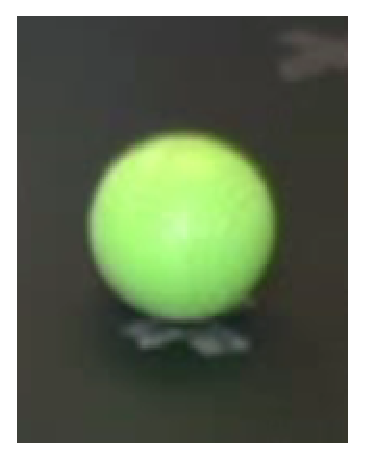
\includegraphics[height=1.75cm]{images/palla}
	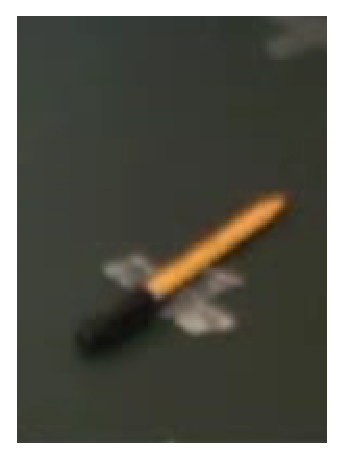
\includegraphics[height=1.75cm]{images/penna}
	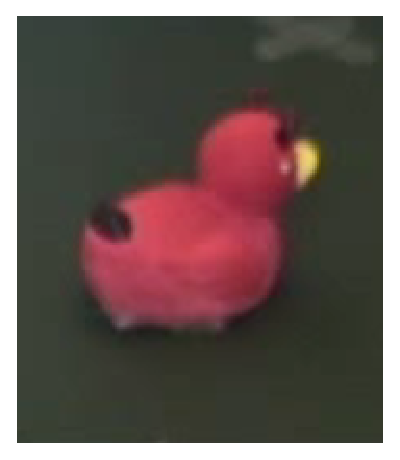
\includegraphics[height=1.75cm]{images/papera}
	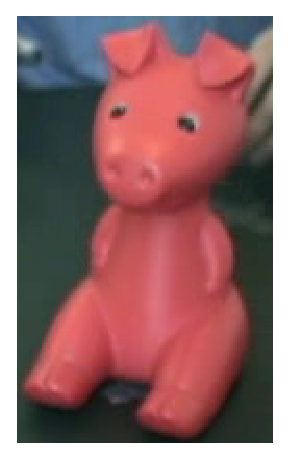
\includegraphics[height=1.75cm]{images/porcellino}
	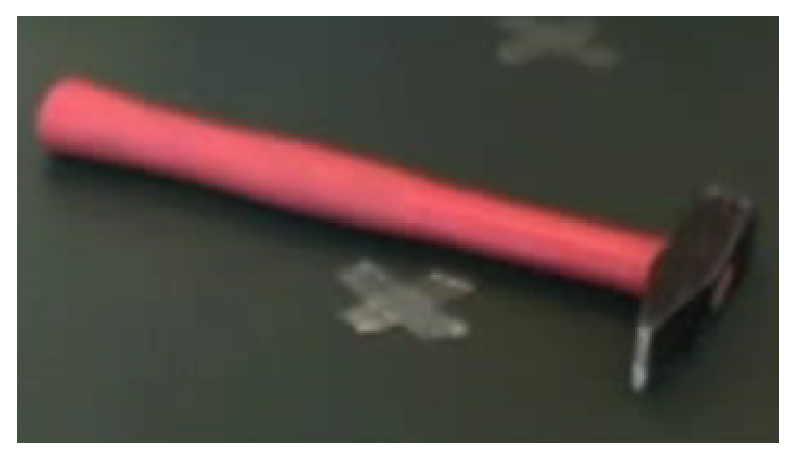
\includegraphics[height=1.75cm]{images/martello}
	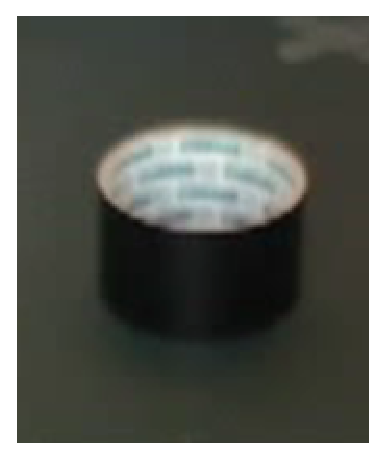
\includegraphics[height=1.75cm]{images/scotch}
	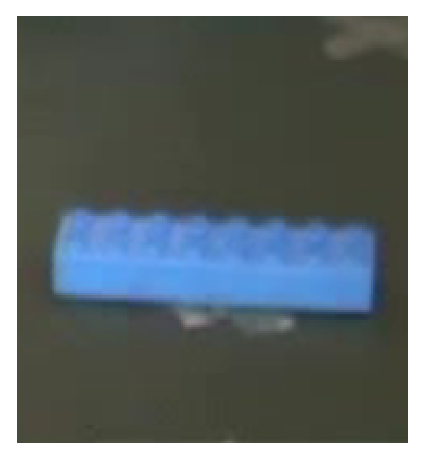
\includegraphics[height=1.75cm]{images/lego}\\
	\vskip 0.1cm
	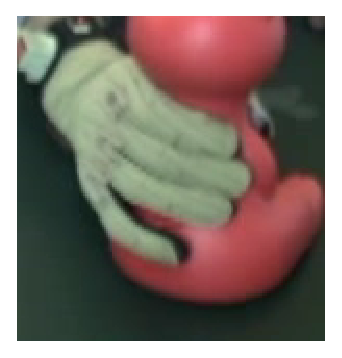
\includegraphics[width=0.19\textwidth]{images/cylinder}
	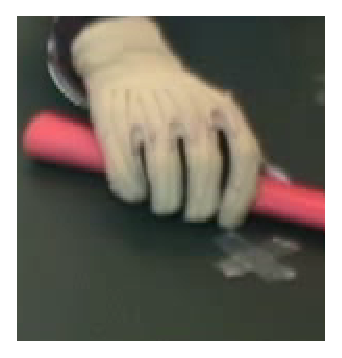
\includegraphics[width=0.19\textwidth]{images/flat}
	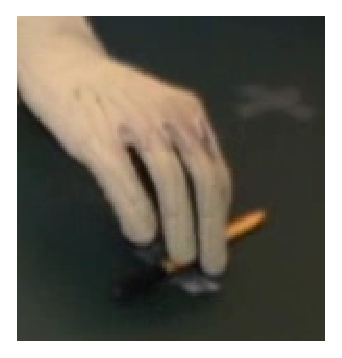
\includegraphics[width=0.19\textwidth]{images/pinch}
	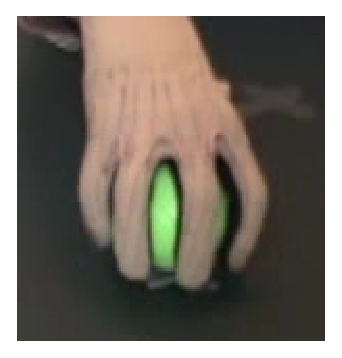
\includegraphics[width=0.19\textwidth]{images/spherical}
	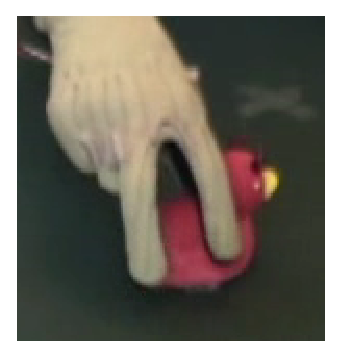
\includegraphics[width=0.19\textwidth]{images/tripodal}
	\caption{Top row: the objects used in our experiments. Bottom, the grasp types we consider: \emph{(left to right)} cylindric power grasp, flat grasp, pinch grip, spherical and
	tripodal grip.}
	\label{fig::grasps}
\end{figure}

The cameras return two video sequences, one placed laterally with focus on the object (the \emph{spectator}) and one placed in front of the subject (observing the \emph{actor}). We process only the {\em spectator} video sequence, because it supplies all the information required for preliminary testing. The video sequence is acquired at $25$Hz by each camera, while the glove is sampled at $100$Hz. Since the three devices are independent of one another a system of common time-stamps was used in order to synchronise the data.\\
The CyberGlove returns $22$ $8$-bit numbers linearly related to the angles of the subject's hand joints. The resolution of the sensors is on average about $0.5$ degree. The sensors describe the position of the three phalanxes of each finger
(for the thumb, rotation and two phalanxes), the four finger-to-finger
abductions, the palm arch, the wrist pitch and the wrist yaw.\\
For these preliminary experiments we considered $7$ objects and $5$ grasping types identified by different hand postures (see Fig. \ref{fig::grasps}); $2$ subjects have joined the experiment: for each object, the actor was asked to perform the required grasping action $20$ times. 

\subsection{Proof of concept experiments}
Among the motor data, it is reasonable to consider only the 22 measures of hand joints as the most relevant for accurately describing the intrinsic properties of each grasping type.
When a grasp occurs the pressure on the force sensing resistor increases, causing the signal to vary hence fixing the time-stamp 
of the event. Concurrently the values on each hand joint are stored as our output data.
%
%We select such data for interesting events (grasping actions) by analysing the signal of the pressure sensor, that assumes lower values when pressure increases.\\
By synchronising motor data and video sequence we select as input data the frames showing an object without clutter, going back along the sequence from the time-stamp in which the event occurs for a fixed amount of frames (see Fig. \ref{fig::vision}, left). 
Our data are thus generated as pairs of image descriptors and sensor-motor values, respectively input and output used to feed the regression model. %In the test phase only the visual information is available.\\ 
The regression methods discussed in Sec.\ref{sec::regression} are implemented in order to predict the expected sensor values of a grasp given the image of an object to be grasped. 
We compare four different image representations, based on bag-of-words descriptors where the histograms are computed for $20$ and $50$ words vocabularies on the entire image or on its four quadrants and then concatenated. We call the representations W20, W20conc, W50 and W50conc.\\
We consider two settings to evaluate the prediction performance of the proposed algorithms. In the first setting (V1-V2) we build training and test sets with the first and second volunteer's data respectively ($140$ examples each). In the second setting (MIXED) we mix the data of both volunteers and perform a 5 fold cross validation (5-CV). For both settings 5-CV on the training data only is used to select the regularizing paramenter for the RLS method and the stopping iteration for the Landweber and $\nu$-method. Tab.\ref{tab:results} summarizes the prediction errors evaluated according to the square loss on all $22$ components.
The prediction errors are consistent among the three learning methods, homogenous with respect to the setting and there are no significant differences among the four representations.
The values for the second setting are markedly lower because mixing the data of both volunteers reduces the variance between training and test sets in each split of the 5-CV. Therefore if we aim at building a model generalizing on several people, it is crucial to collect data from a large variety of volunteers.\\
\begin{table}[h!]
\centering
\begin{tabular}{|c|c|c|c|c|}
\hline Setting & Representation  & RLS $[10^3]$ & Land $[10^3]$ & Nu $[10^3]$\\\hline
\multirow{4}{*}{V1-V2} & W20conc  & $48$ & $47$& $47$\\\cline{2-5}
&W20  	  & $37$ & $38$& $38$\\\cline{2-5}
&W50conc & $41$ & $40$& $40$\\\cline{2-5}
&W50 	  & $43$ & $43$& $43$\\\hline
\multirow{4}{*}{MIXED} 
& W20conc & $6.1 (1.1) $ & $6.4 (1.2) $& $6.4 (1.2) $\\\cline{2-5}
& W20 & $7.9 (1.3) $ & $8.0 (1.2) $& $8.0 (1.3) $\\\cline{2-5}
&  W50conc &   $6.1 (0.8) $ & $6.1 (0.9) $& $6.3 (0.7) $\\\cline{2-5}
& W50 & $7.4 (2.0) $ & $7.2 (2.0) $& $7.3 (2.0) $\\\hline
\end{tabular}
\caption{Prediction accuracies of the proposed methods for the two settings and four representations. The accuracy is expressed as 
mean square error. In the MIXED scenario the associated variance is reported as well.}
\label{tab:results}
\end{table}
Finally, we aim at classifying the grasp type given the estimated sensor values.
We restrict at the MIXED setting, using the best regression outcome case,  W50conc/RLS.
The input data are the sensor measures and the output data are the grasp classes.
Again, a 5-CV is performed. For each split the training set is the actual set of measures from the sensors paired with the corresponding
grasp type, while the test set is the set of estimated measures.  
We train a RLS classifier \cite{rifkin03rlsc} in a One-vs-All configuration 
 obtaining a prediction accuracy of 99.6 (0.8)\%. 
 This result indicates that the regression models perform well and 
 guaranteeing the validity of the idea underlying the framework.











\section{Discussion and future work}
In this paper we proposed a general architecture for learning multi-modal patterns of data. 
The underlying assumption is that the system we want to model has several perceptual channels available, 
but among them some might be inactive. 
We adopted a regression-based approach to build a behavioral model of the system 
that can be exploited to amend such inactivity.
As a validation attempt, we presented an application for grasp prediction by means of vector 
valued regression: the experimental phase produced very promising results that encourage 
us to further investigate this framework. 
Even though the regression problem is inherently vector-valued, we  restricted 
our analysis to the simple scalar-valued case. 
A preliminary analysis on the covariance matrix of the sensors measures 
shows some correlation among the sensors, both positive and negative, 
pointing at the usefulness of a full-fledged vector-valued approach. 
Recently, much work has been devoted on how to best exploit the similarity among the components 
and learn all of them simultaneously. The main idea behind most of the literature is to use prior 
knowledge on the components relatedness to design a particular penalization term or a proper 
matrix-valued kernel \cite{micchelli04kernels}. 
In absence of prior knowledge, one approach is to design an heuristic to evaluate the similarity 
among the components from the available data, e.g. by computing the sample covariance of the 
sensor measures. 
Our current research is focused on how to translate this information into a viable matrix-valued kernel. 
Alternatively one can learn the vector structure directly in the training phase 
\cite{pontil08transferlearning,jacob08clusteredmtl}.  

This  multifaceted framework can be further extended in different directions. 
Regarding the experimental setup, we plan to enrich the dataset with a higher number of subjects, and multiple grasps for each object. Indeed, this will let us relax the one-to-one assumption we adopted in this paper and investigate a more realistic many-to-many mapping between objects and grasp classes.
As anticipated in the introduction, the modeled mapping will be used in the context of multimodal learning to investigate whether, by reconstructing a missing modality, the object recognition rate improves.
From the statistical learning viewpoint, we plan to explore new solutions drawing inspiration from the mentioned works on multitask learning. 

\subsection*{Acknowledgments}
This work was supported by the EMMA project sponsored by the Hasler Foundation (B. C.)

\begin{thebibliography}{4}

\bibitem{rizz} Rizzolatti, G., Craighero, L.: The Mirror-Neuron System. Annual Review of Neuroscience. 27:169-92 (2004)

\bibitem{harris} Harris, C., Stephens, M.: A Combined Corner and Edge Detector. Proceedings of The Fourth Alvey Vision Conference. pp. 147-151 (1988)

\bibitem{schmid} Mikolajczyk, K., Schmid, C.:Scale and Affine Invariant Interest Point Detectors. In IJC. V 60(1):63-86 (2004)

\bibitem{lowe} Lowe, D. G.: Distinctive Image Features from Scale-Invariant Keypoints. International Journal of Computer Vision. 60 (2): 91-110 (2004) 

%\bibitem{lindeberg} Lindeberg, T.: Feature Detection with Automatic Scale Selection. International Journal of Computer Vision. 30 (2): 79–116 (1998)

%\bibitem{perona} Moreels, P., Perona, P.: Evaluation of Features Detectors and Descriptors Based on 3D Objects. In ICCV. (2005)

\bibitem{schmid2} Mikolajczyk, K., Schmid, C.:A Performance Evaluation of Local Descriptors. Trans on PAMI. 27(10) (2005)

%\bibitem{leibe} Leibe, B., Mikolajczyk, K., Schiele, B.: Efficient Clustering and Matching for Object Class Recognition. In BMVC. (2006)

\bibitem{csurka} Csurka, G., Dance, C.R., Fan, L., Bray, C.: Visual Categorization with Bag of Keypoints. In ECCV. (2004)

\bibitem{ferrari} Ferrari, V., Tuytelaars, T., Van Gool, L.: Simultaneous Object Recognition and Segmentation from Single or Multiple Model Views. IJVC. 67(2) (2006)

\bibitem{LoGerfo08Spectral} Lo Gerfo, L., Rosasco, L., Odone, F., De Vito, E., Verri, A.:
  Spectral Algorithms for Supervised Learning. Neural Computation. 20(7) (2008)

 \bibitem{Yao07Early}
   Yao, Y., Rosasco, L., Caponnetto, A.: On Early Stopping in Gradient Descent Learning.
   Constructive Approximation. 26(2) (2007)

\bibitem{MicchPon05Onlearning} Micchelli, C.~A., Pontil, M.: On learning vector-valued functions.
  Neural Computation. 17 (2005)

\bibitem{dev04representer} De Vito, E., Rosasco, L., Caponnetto, A., Piana, M.,	Verri, A.:Some Properties of Regularized Kernel Methods. Journal of Machine Learning Research. 5 (2004)

\bibitem{preprint} Baldassarre, L., Barla, A.,  Rosasco, L., Verri, A.:
Learning vector valued functions with spectral regularization. (preprint)

% \bibitem{jung} Hye-Won, J., Yong-Ho, S., Ryoo, M.S., Yang, H.S: Affective Communication System with Multimodality for a Humanoid Robot, AMI.
% 4th IEEE/RAS International Conference on Humanoid Robots. 2 (2004)

% \bibitem{kruger} Kr$\ddot{u}$ger, N., Felsberg, M., W$\ddot{o}$rg$\ddot{o}$tter, F.: Processing Multi-modal Primitives from Image Sequences. 4th ICSE Symposium on Engineering of Intelligent Systems. (2004) 

% \bibitem{yang} Yang, G., Lin, Y., Bhattacharya, P.: Multimodality Inferring of Human Cognitive States Based on Integration of Neuro-Fuzzy Network and Information Fusion Techniques. EURASIP Journal on Advances in Signal Processing. 8(2008)

\bibitem{gallese} Gallese, V., Fadiga, L., Fogassi, L., Rizzolatti, G.: Action Recognition in the Premotor Cortex. Brain. 119, 593-609 (1996)

% \bibitem{grans} Granström, B. House, D., Karlsson, I.: Multimodality in Language and Speech Systems. Text, Speech and Language Technology. 19(2002)

\bibitem{metta} Metta, G., Sandini, G., Natale, L., Craighero, L., Fadiga, L.: Understanding  Mirror Neurons: A Bio-Robotic Approach. Interaction Studies. 7, 197-232, (2006)

% \bibitem{caputo} Luo, J., Pronobis, A., Caputo, B.: SVM-based Transfer of Visual Knowledge Across Robotic Platforms. 5th International Conference on Computer Vision Systems. (2007)

% \bibitem{thrun} Thrun, S., Mitchell, T.: Lifelong Robot Learning. Robotics and Autonomoues Systems. 15 (1995)

% \bibitem{malak} Malak, R.J., Khosla, P.K.: A Framework for the Adaptive Trasfer of Robot Skill Knowledge Using Reinforcement Laerning Agents. Proc of ICRA. (2001)

% \bibitem{barto} Konidaris, G., Barto, A.G.: Autonomous Shaping: Knowledge Transfer in Reinforcement Learning. Proc. of ICML. (2006) 

\bibitem{wong} Hartigan, J. A., Wong, M. A.: A K-Means Clustering Algorithm". Applied Statistics. 28(1) (1979) 

\bibitem{cutkosky} Cutkosky, M.: On grasp choice, grasp models and the design of hands for manufacturing tasks. IEEE Transactions on Robotics and
Automation. (1989)

\bibitem{2007.AR} Castellini, C., Orabona, F., Metta, G., Sandini, G.: Internal Models of Reaching and Grasping. Advanced Robotics. 21(13) (2007)

%\bibitem{papcun} Papcun, G., Hochberg, J., Thomas, T. R., Laroche, F., Zacks, J., Levy, S.: Inferring articulation and recognizing gestures from acoustics with a neural network trained on x-ray microbeam data. J Acoust Soc Am. 92(2) (1992)

%\bibitem{richmond} Richmond, K., King, S., Taylor, P.: Modelling the uncertainty in recovering articulation from acoustics. Computer Speech and Language. 17 (2003)

\bibitem{bulmann02boosting} Buhlmann, P.: Boosting for High-Dimensional Linear Models". Annals of Statistics. 34(2),  (2006)

\bibitem{micchelli04kernels} Micchelli, C. A., Pontil, M.: Kernels for Multi-task Learning. NIPS (2004)

\bibitem{rifkin03rlsc} Rifkin, R., Yeo, G., Poggio, T.: Regularized Least-Squares Classification. Advances in Learning Theory: Methods, Models and Applications. (2003) 

\bibitem{pontil08transferlearning} Argyriou, A., Maurer, A., Pontil, M.: An Algorithm for Transfer Learning in a Heterogeneous Environment. ECML/PKDD. (1) 71-85 (2008) 

\bibitem{jacob08clusteredmtl} Jacob, L., Bach, F., Vert, J.P.: Clustered Multi-Task Learning: a Convex Formulation. NIPS. (2008) 

\end{thebibliography}

\end{document}
